\documentclass[10pt,journal,compsoc]{IEEEtran}
\usepackage{xeCJK}

% *** CITATION PACKAGES ***
%
\ifCLASSOPTIONcompsoc
  % IEEE Computer Society needs nocompress option
  % requires cite.sty v4.0 or later (November 2003)
  \usepackage[nocompress]{cite}
\else
  % normal IEEE
  \usepackage{cite}
\fi

\begin{document}

\title{网络游戏中收集任务的概率问题}

\author{15211068~谭伟豪~~15211063~于牧之}

\maketitle

\newtheorem{definition}{Definition}
\renewcommand{\abstractname}{摘 要}
\renewcommand{\figurename}{图}
\renewcommand{\tablename}{表}
\renewcommand{\IEEEkeywordsname}{关键词}
\begin{abstract}
收集式游戏中常常存在“还需要获得多少物品才能达到我的收集目标”这一问题,我们通过对游戏中的收集过程进行数学建模,从而定量地考察了一个游戏中想要完成收集目标的难度。
\end{abstract}
\renewcommand{\abstractname}{Abstract}
\begin{abstract}
The effort of achieving the goals in collectible games is worth noting. 
\end{abstract}

\begin{IEEEkeywords}
概率, 收集式游戏, 赌博.
\end{IEEEkeywords}
\renewcommand{\IEEEkeywordsname}{Keywords}
\begin{IEEEkeywords}
Probability, Collectible Game, Gambling.
\end{IEEEkeywords}

\section{引言}

目前市面上的网络游戏大多带有收集要素,如《地下城与勇士》中需要收集装备来提高自己的战斗力,《阴阳师》中需要收集式神来优化自己的出战阵容。对于这类游戏来说,“通关”很大程度上依赖于收集任务的完成度。

游戏的收集要素往往带有极大的不确定性,获得一件物品时,它的种类、稀有度等等属性很多时候是随机的。对于玩家来说,往往只能在



\section{定义}

本节我们将探讨关于游戏中的收集任务的一些定义,以便后续讨论。

\begin{definition}
  物品(Item)
\end{definition}

\section{模型的建立}

针对上面的研究问题,我们可以对迁移学习的情境和方法进行分类。

\begin{table*}[!ht]
\centering
\caption{迁移学习的方法}
\label{tab:survey_method}
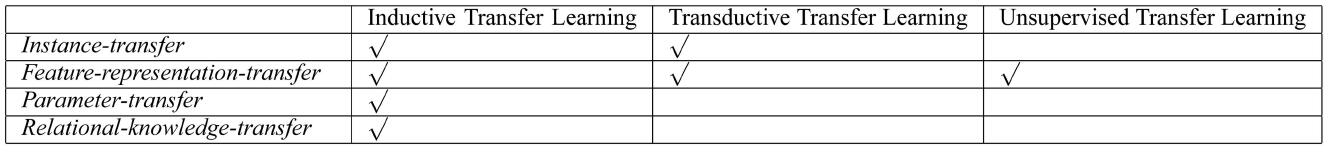
\includegraphics[width=40pc]{img/survey_tab3.jpg}
\end{table*}

\begin{figure*}[!ht]
\centering
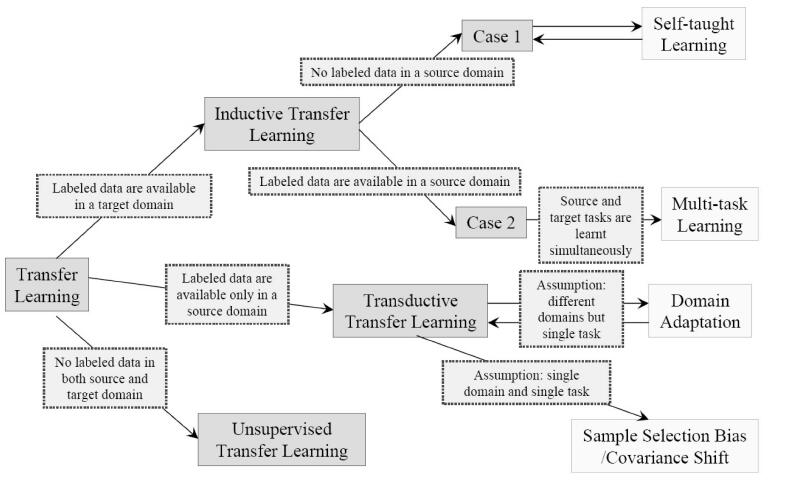
\includegraphics[width=30pc]{img/survey_fig1.jpg}
\caption{迁移学习方法与情境的关系}
\label{fig:survey_method}
\end{figure*}


\begin{enumerate}
\item 在归纳迁移的情境中,目标任务和源任务是不同的,而目标域和源域可能相同也可能不同。此类问题中,目标域中必须要有带标签的数据才能训练出目标预测模型$f_T(\cdot)$。根据源域中无标签数据和标签数据的情形不同,我们还能进一步将归纳迁移算法分为这样两类:\\
a. 源域中有很多标签数据。此时归纳迁移算法类似于多任务学习算法。但区别在于,前者更侧重于在目标问题中取得更好的性能,而后者则试图同时完成源任务和目标任务。\\
b. 源域中无标签数据。此时归纳学习算法比较接近自学(self-taught learning)算法。因为在自学算法的使用场景中源任务和目标任务的标签空间可能不同,而这与源域中无标签数据的情形是很近似的。

\item 在转导学习的情境中,目标任务和源任务是一样的,但源域和目标域是不同的。这种情况下目标域是没有标签数据的,但源域有很多。根据源域和目标域之间的区别,我们还能进一步将转到学习的情境划分为这样两类:\\
a. 二者的特征空间不同$X_S \ne X_T$\\
b. 特征空间相同$X_S \ne X_T$,但边缘概率分布不同,$P(X_S) \ne P(X_T)$\\
后者和文本分类中的域适应很相似,因为他们的基本假设是一样的。
\item 最后,还有无监督迁移学习的情境。它与归纳迁移学习的情境类似,目标问题和源问题不同但相关。区别在于,无监督迁移学习中目标问题是无监督问题,如聚类、降维等。在此情境中,源域和目标域都没有带标签的数据。
\end{enumerate}




\section{结论}

地下城与勇士没有妹子好玩。

\bibliographystyle{IEEEtran}
\bibliography{thesis}

\end{document}
